\documentclass{beamer}
\usepackage[utf8]{inputenc}
\usepackage[T1]{fontenc}
\usetheme{metropolis}
\usepackage[finnish]{babel}
\usepackage{graphicx}
\usepackage{tabularx}
\usepackage{hyperref}
\setbeameroption{show notes}


\title{Lajirikkauskartta}
\author{\parbox{\textwidth}{Konsta Happonen\\
    Open Knowledge Finland\\
    \\
    \href{http://twitter.com/koalha}{@Koalha}\\
    \url{lajirikkauskartta.fi}}\\
    \\
    \textbf{CC-BY 4.0}
}
\date{}
\usebackgroundtemplate{
\includegraphics{light-grey-rgb.pdf}}

\begin{document}
\maketitle

\begin{frame}{Tausta}
  Suomi on metsärikas maa.

  Ihmiset kuitenkin arvostavat metsiä eri syistä: materiaalina, energianähteenä, virkistysalueina ja itseisarvoisina luontokohteina

  \vspace{1cm}
  
  \Huge $\rightarrow$ Metsäkonfikteja

\end{frame}


\begin{frame}{Projektin tausta}
\begin{figure}
\subfloat{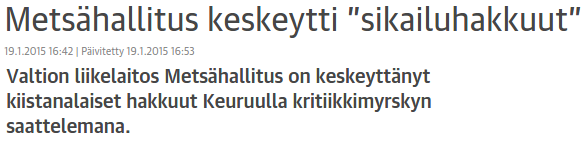
\includegraphics[width=7cm]{otsikot.png}}
\subfloat{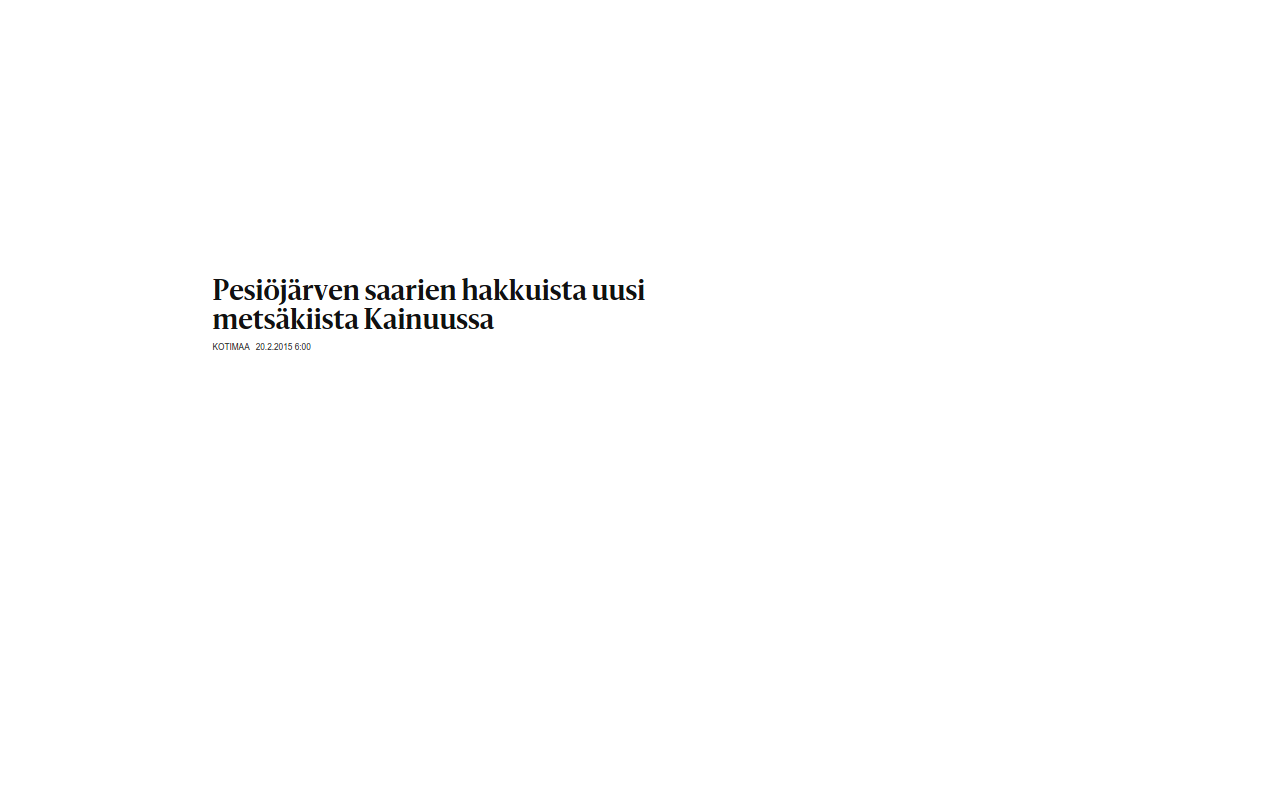
\includegraphics[width=5cm]{otsikot2.png}}
\end{figure}

\begin{figure}
\subfloat{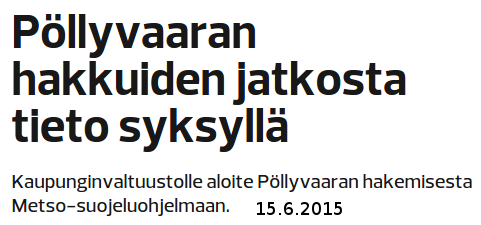
\includegraphics[width=5cm]{otsikot3.png}}
\subfloat{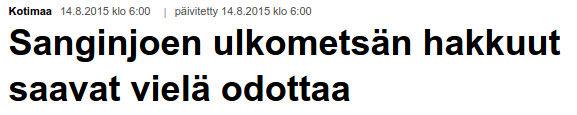
\includegraphics[width=5cm]{otsikot4.png}}
\end{figure}

\end{frame}


\begin{frame}{Aineistot}
  MML:n laserkeilausaineistot

  Ympäristöhallinon vanhojen metsien suojelualueiden rajaukset

  Suomen metsäkeskukselta rajaukset metsätalouskäytössä olevista alueista
  
\end{frame}

\begin{frame}{Laserkeilausaineistot}
  \begin{center}
    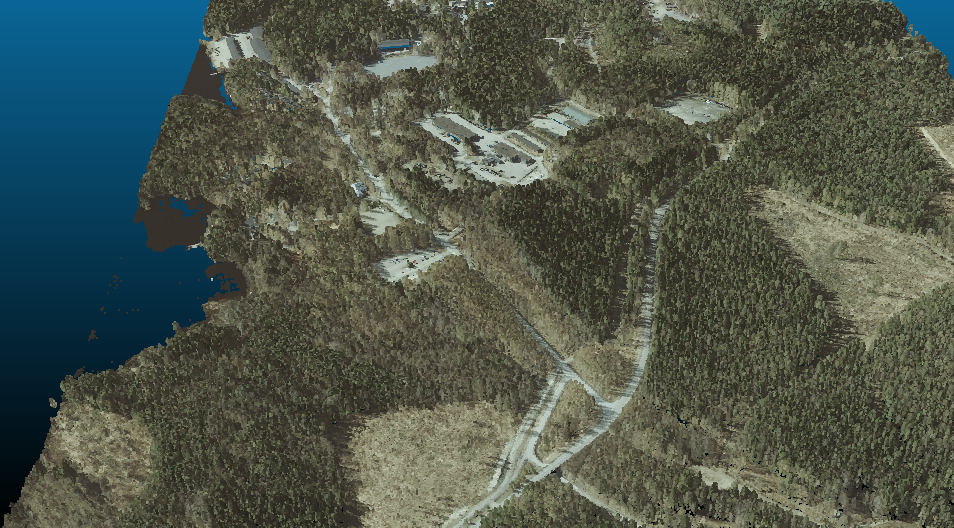
\includegraphics[width=\textwidth]{laasereita.png}
  \end{center}
\end{frame}

\begin{frame}{Laserkeilausaineistot}
  \begin{center}
    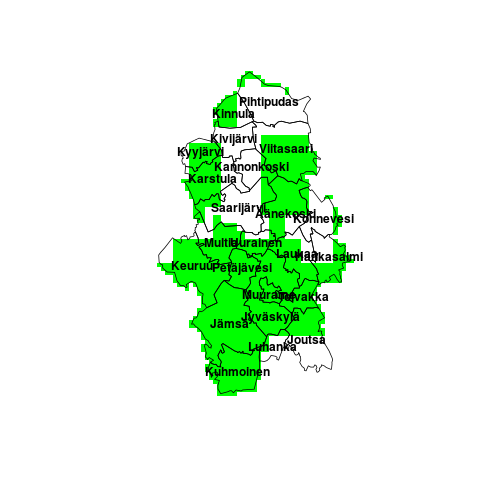
\includegraphics[height=0.9\textheight]{laserkattavuus.png}
  \end{center}
\end{frame}

\begin{frame}{Suojelualuerajaukset}
  \begin{center}
    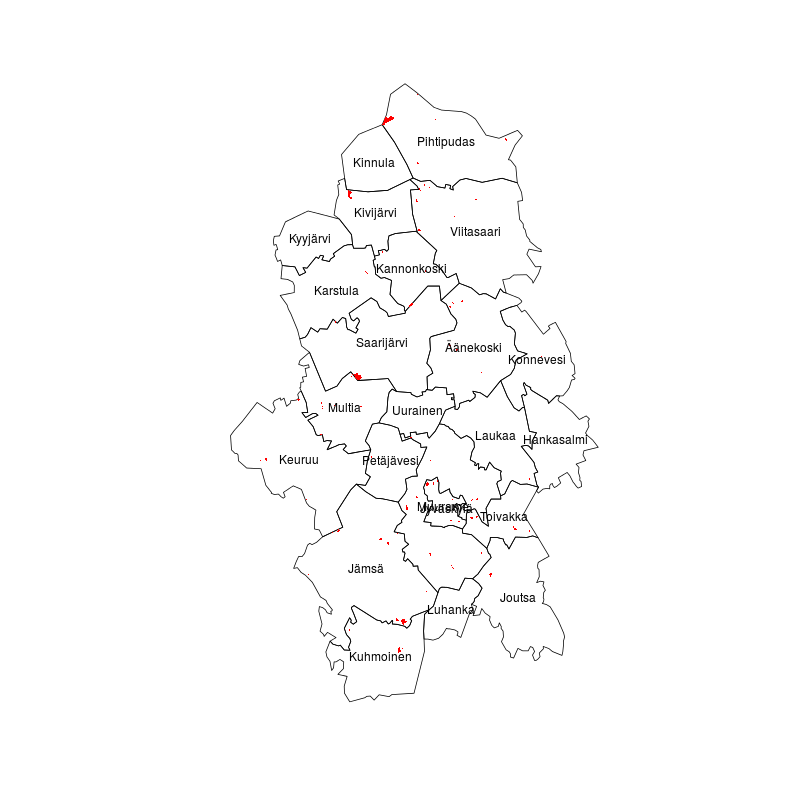
\includegraphics[height=0.9\textheight]{suojelualueet.png}
  \end{center}
\end{frame}

\begin{frame}{Metsämaski}
  \begin{center}
    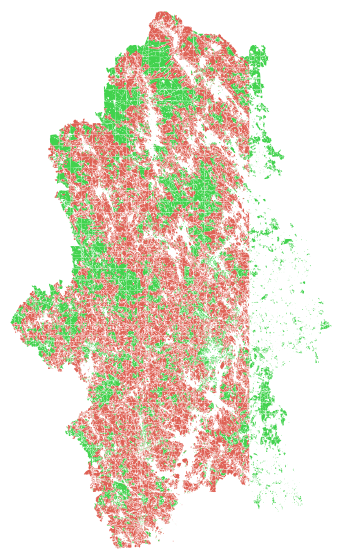
\includegraphics[height=0.9\textheight]{maski.png}
  \end{center}
\end{frame}

\begin{frame}{Menetelmät}
  Pistepilvien muuttaminen metsän rakennetta kuvaaviksi muuttujiksi

  MaxEnt - mallin opettaminen vanhan metsän suojelualueilla

  Suojelualueiden kaltaisten, vielä suojelettomien metsien ennustaminen kartalle 
\end{frame}

\begin{frame}{Metsän rakennemuuttujat}
  \begin{center}
    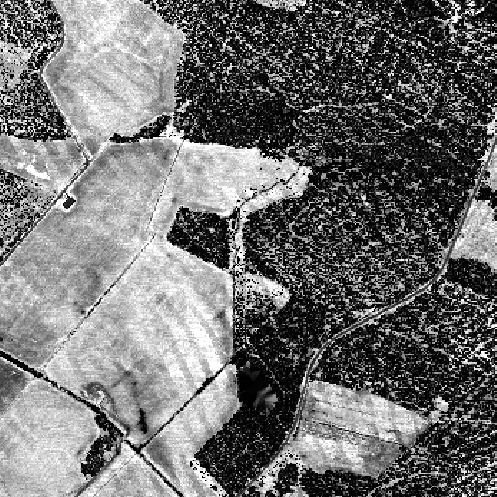
\includegraphics[height=0.9\textheight]{intensity.png}
  \end{center}
\end{frame}


\begin{frame}{Metsän rakennemuuttujat}
  \begin{center}
    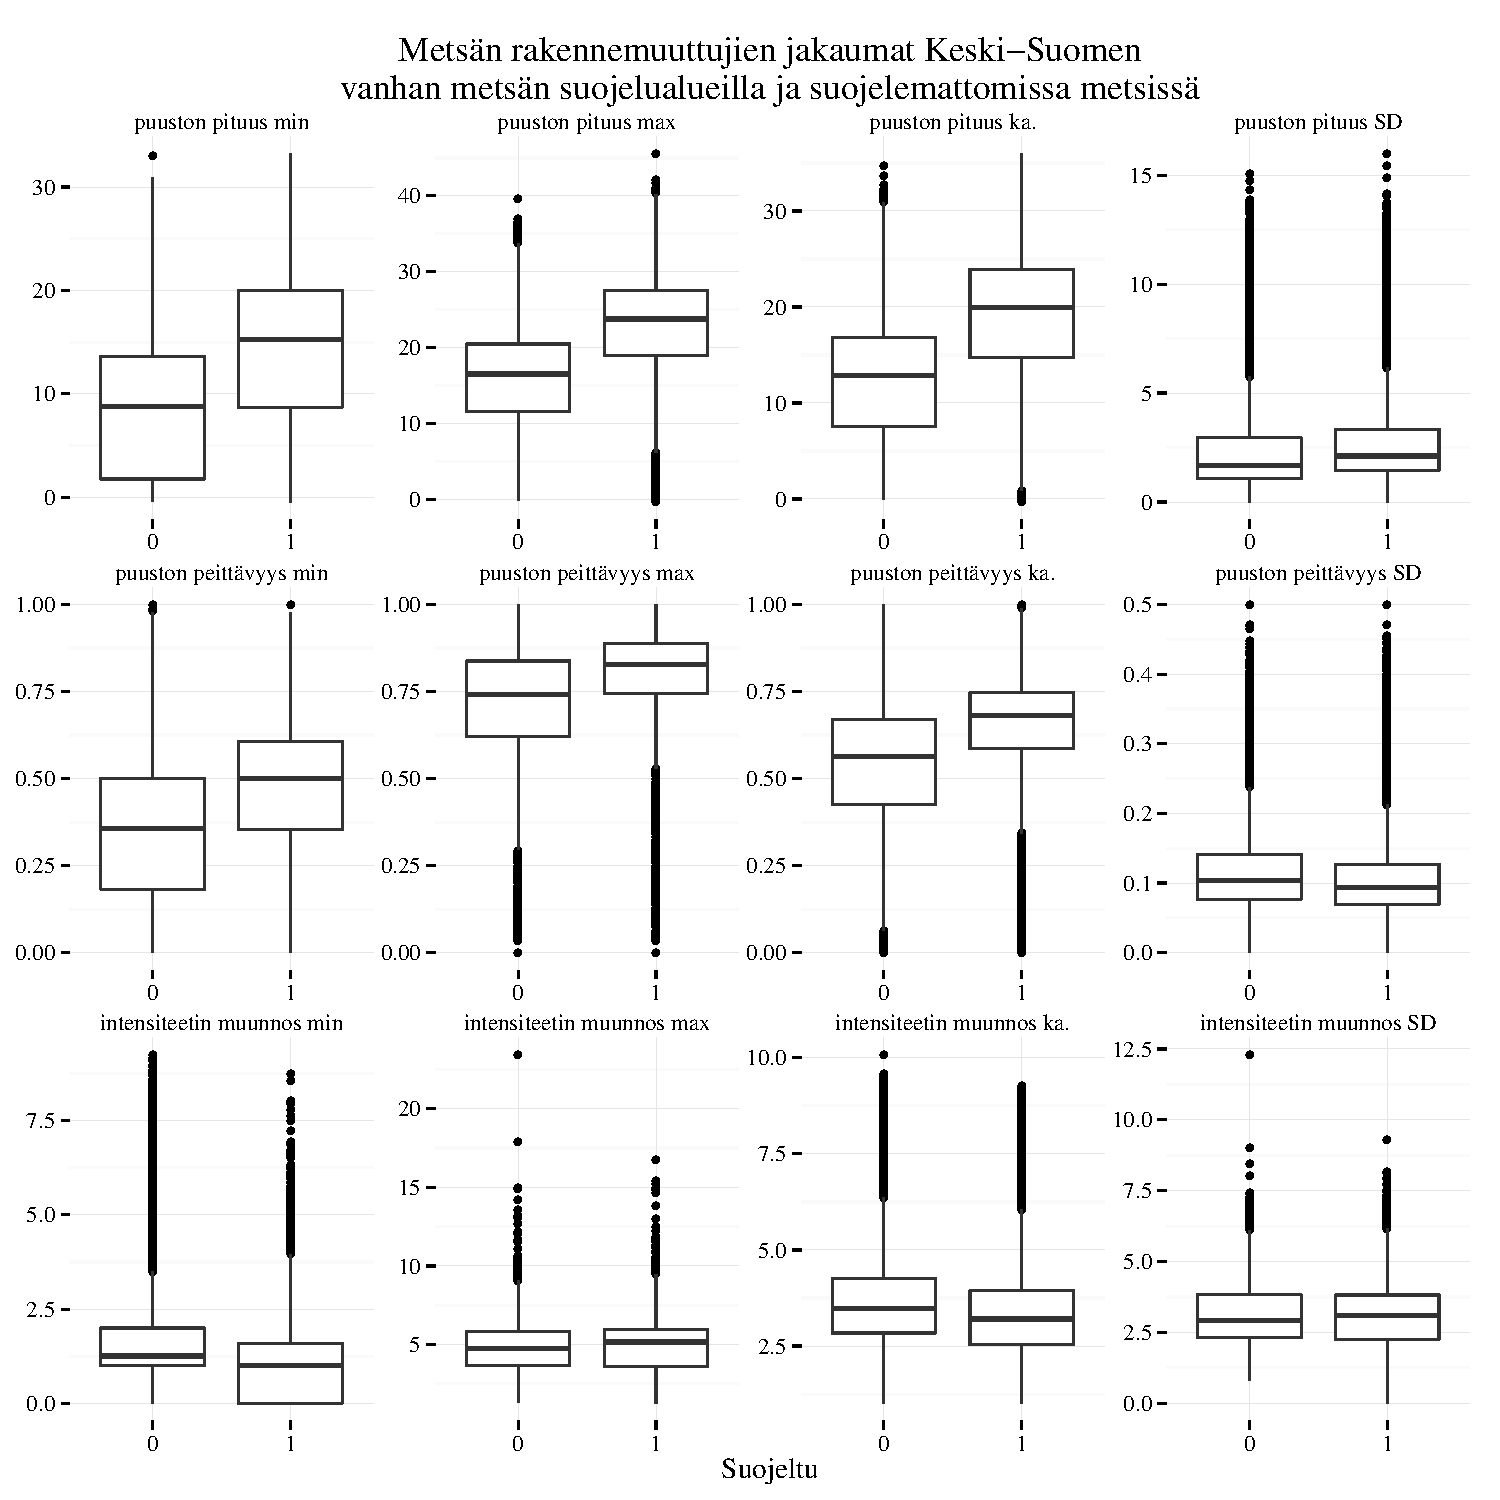
\includegraphics[height=0.9\textheight]{metsamuuttujien_jakaumat.pdf}
  \end{center}
\end{frame}

\begin{frame}{MaxEnt-malli}
  \begin{center}
    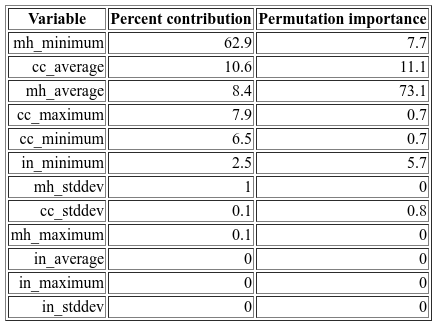
\includegraphics[height=0.9\textheight]{maxent.png}
  \end{center}
\end{frame}

\begin{frame}{Validointi}
   \begin{center}
    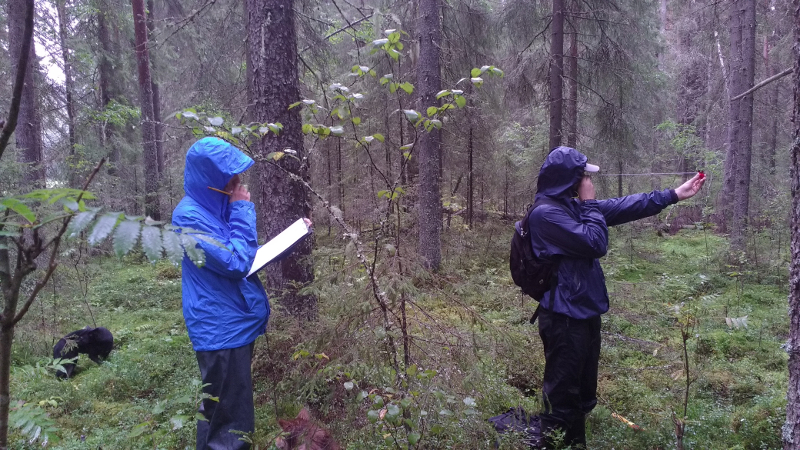
\includegraphics[width=\textwidth]{validointi2.jpg}
  \end{center}
\end{frame}

\begin{frame}{Validointi}
   \begin{center}
    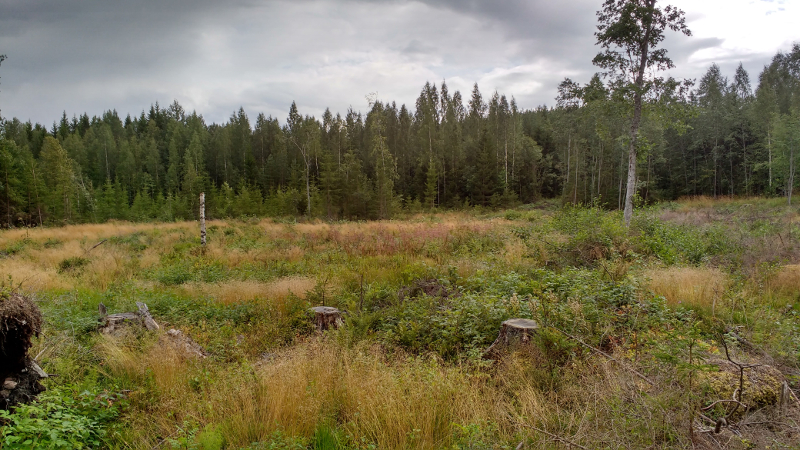
\includegraphics[width=\textwidth]{validointi1.jpg}
  \end{center}
\end{frame}


\begin{frame}{Tulokset}
  Pohjapinta-ala, elävät ja kuolleet puut

  Maapuiden määrä, biomassa ja lahoaste
\end{frame}

\begin{frame}{Tulokset}
  \begin{center}
    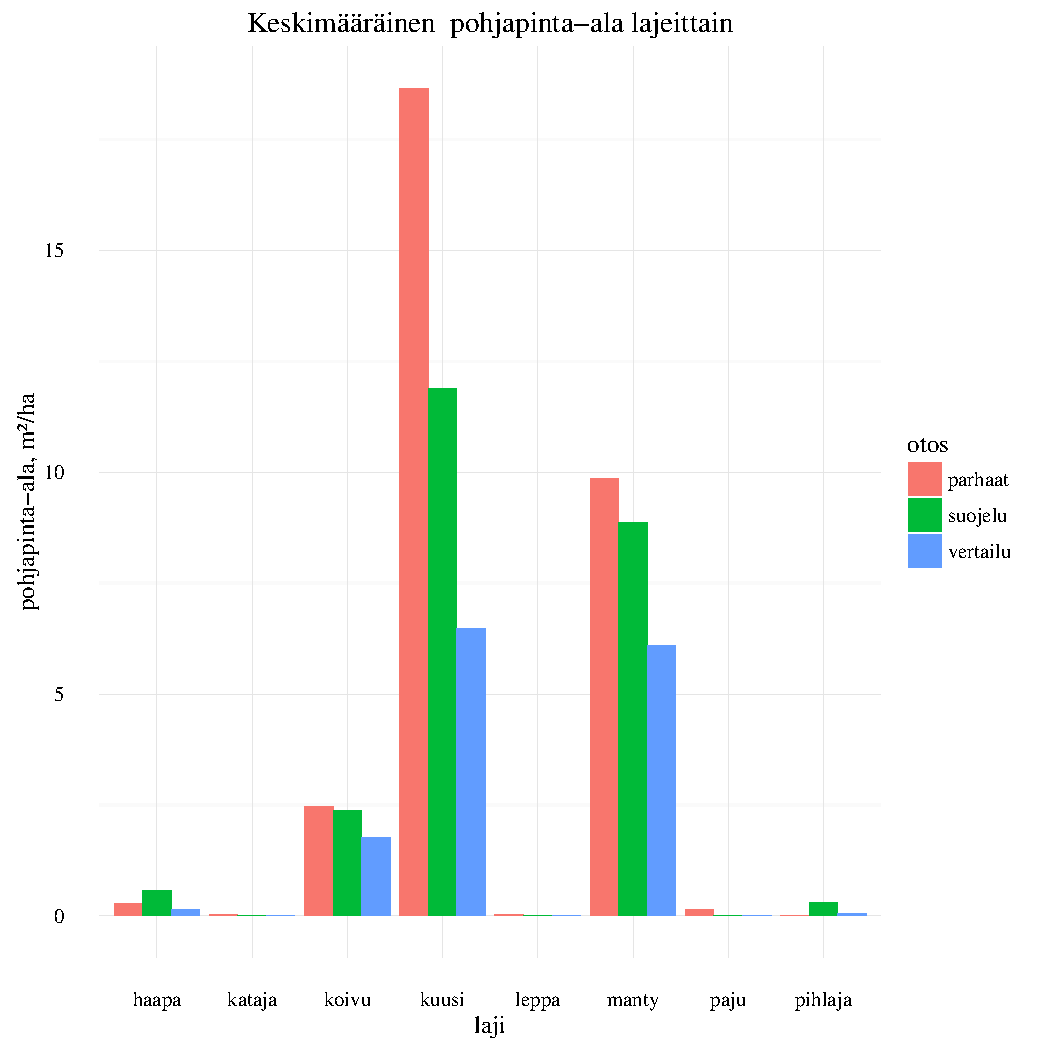
\includegraphics[height = 0.9\textheight]{pohja-ala.pdf}
  \end{center}
\end{frame}

\begin{frame}{Tulokset}
  \begin{center}
    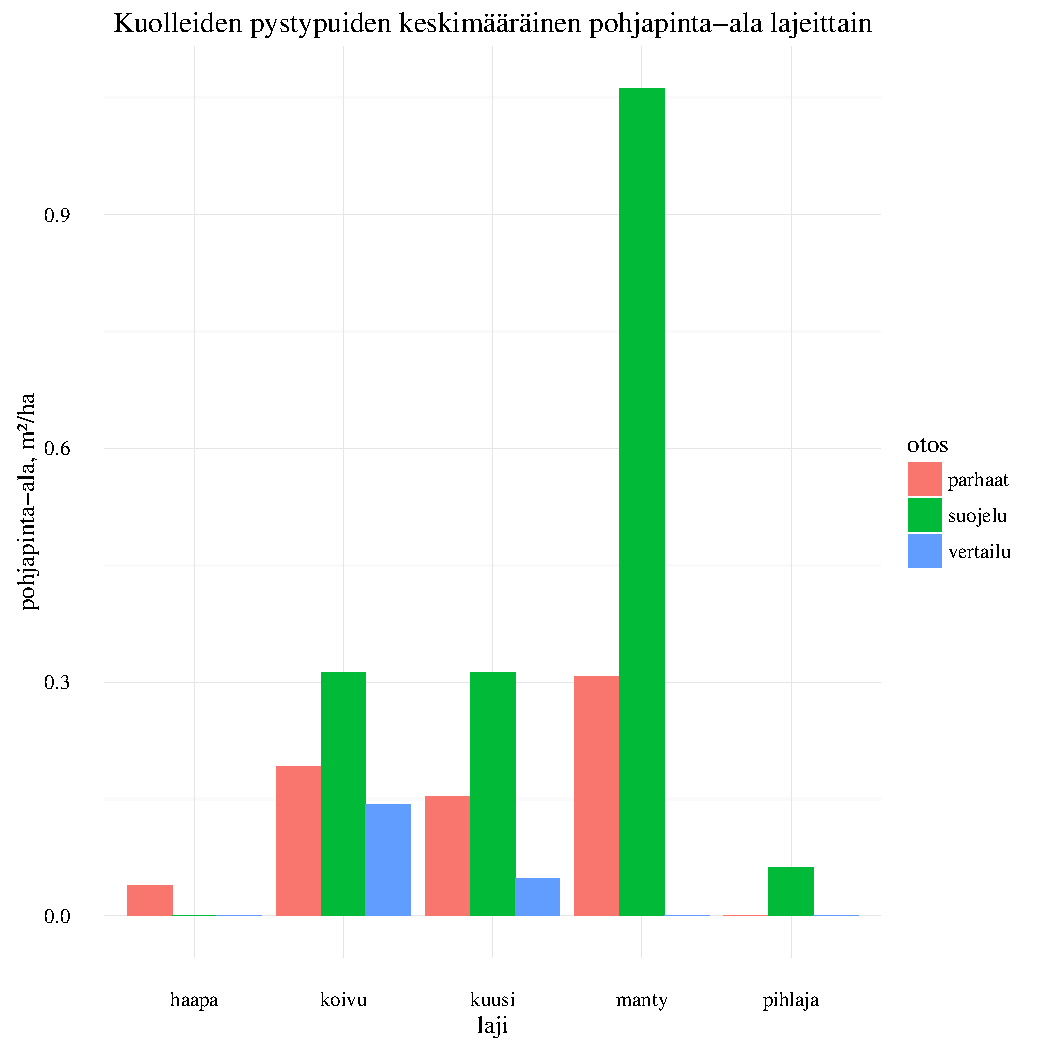
\includegraphics[height = 0.9\textheight]{pystypuut.pdf}
  \end{center}
\end{frame}

\begin{frame}{Tulokset}
  \begin{center}
    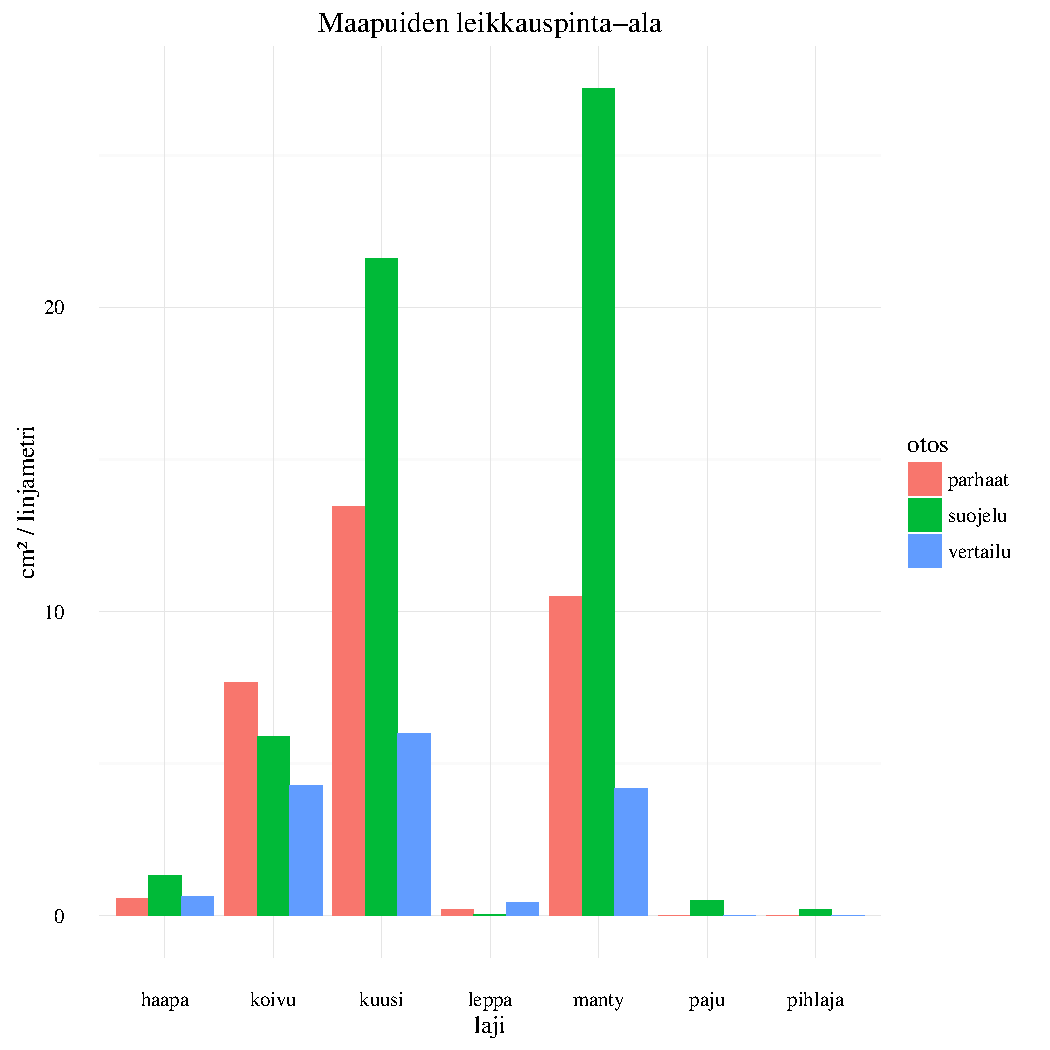
\includegraphics[height = 0.9\textheight]{maapuut.pdf}
  \end{center}
\end{frame}

\begin{frame}{Tulokset}
  \begin{center}
    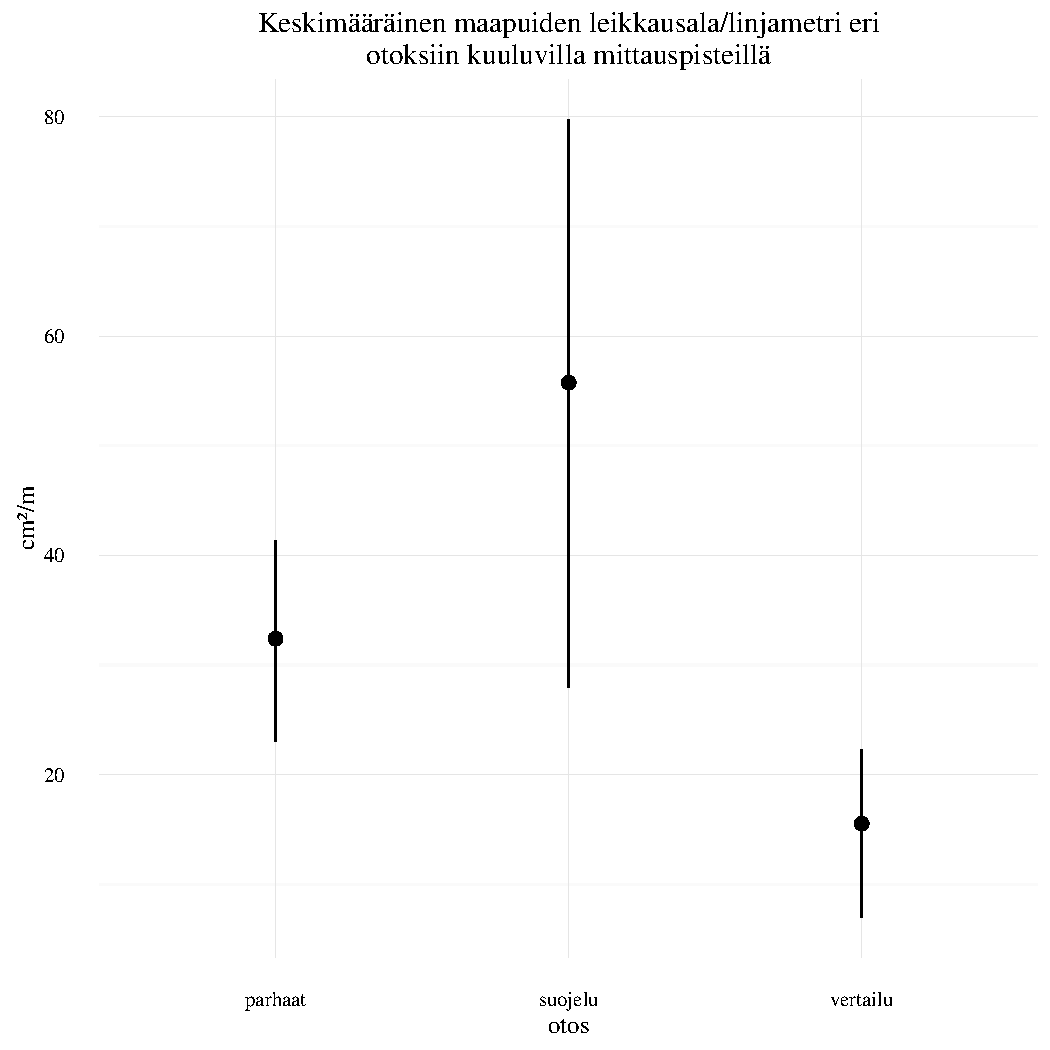
\includegraphics[height = 0.9\textheight]{maapuiden_leikkausala_boot.pdf}
  \end{center}
\end{frame}

\begin{frame}{Tulokset}
  \begin{center}
    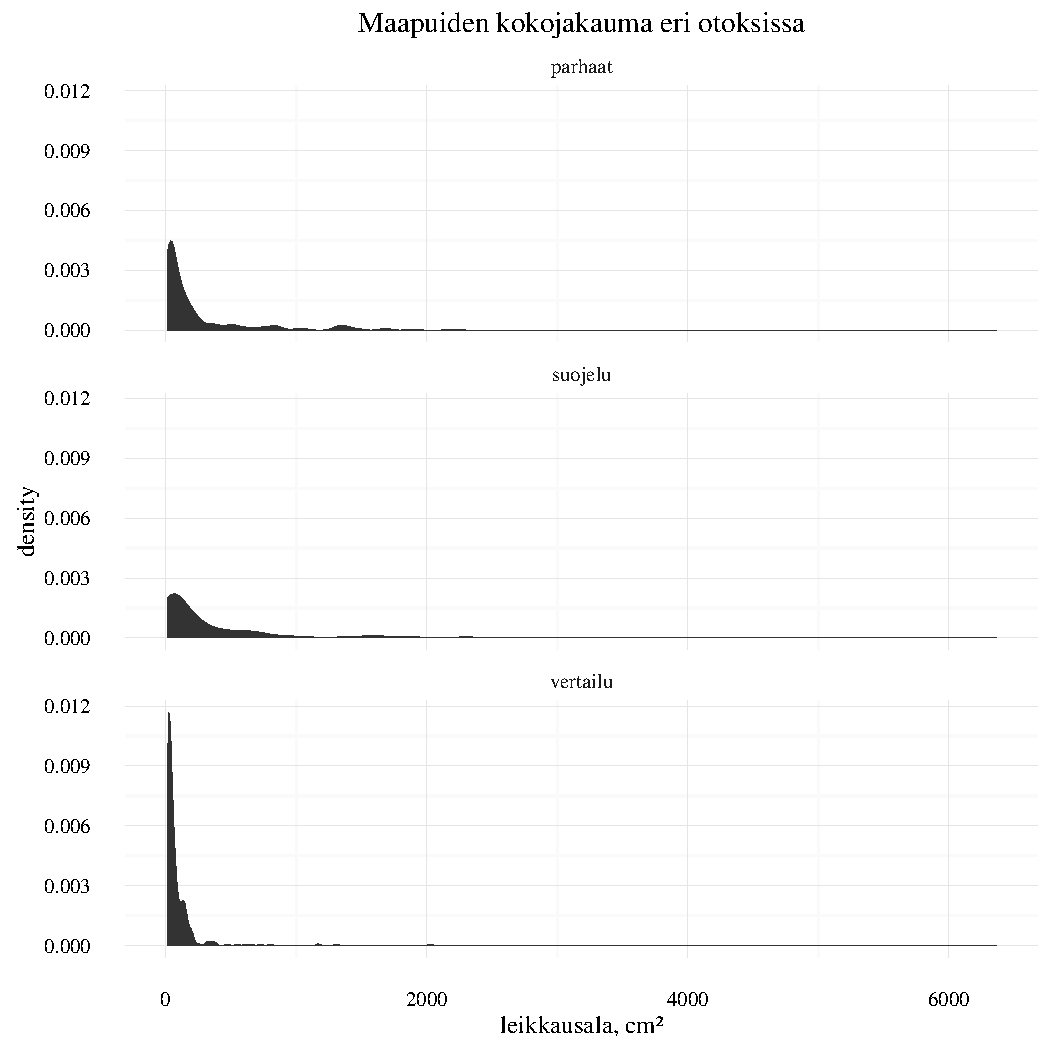
\includegraphics[height = 0.9\textheight]{maapuiden_koko.pdf}
  \end{center}
\end{frame}

\begin{frame}{Tulokset}
  \begin{center}
    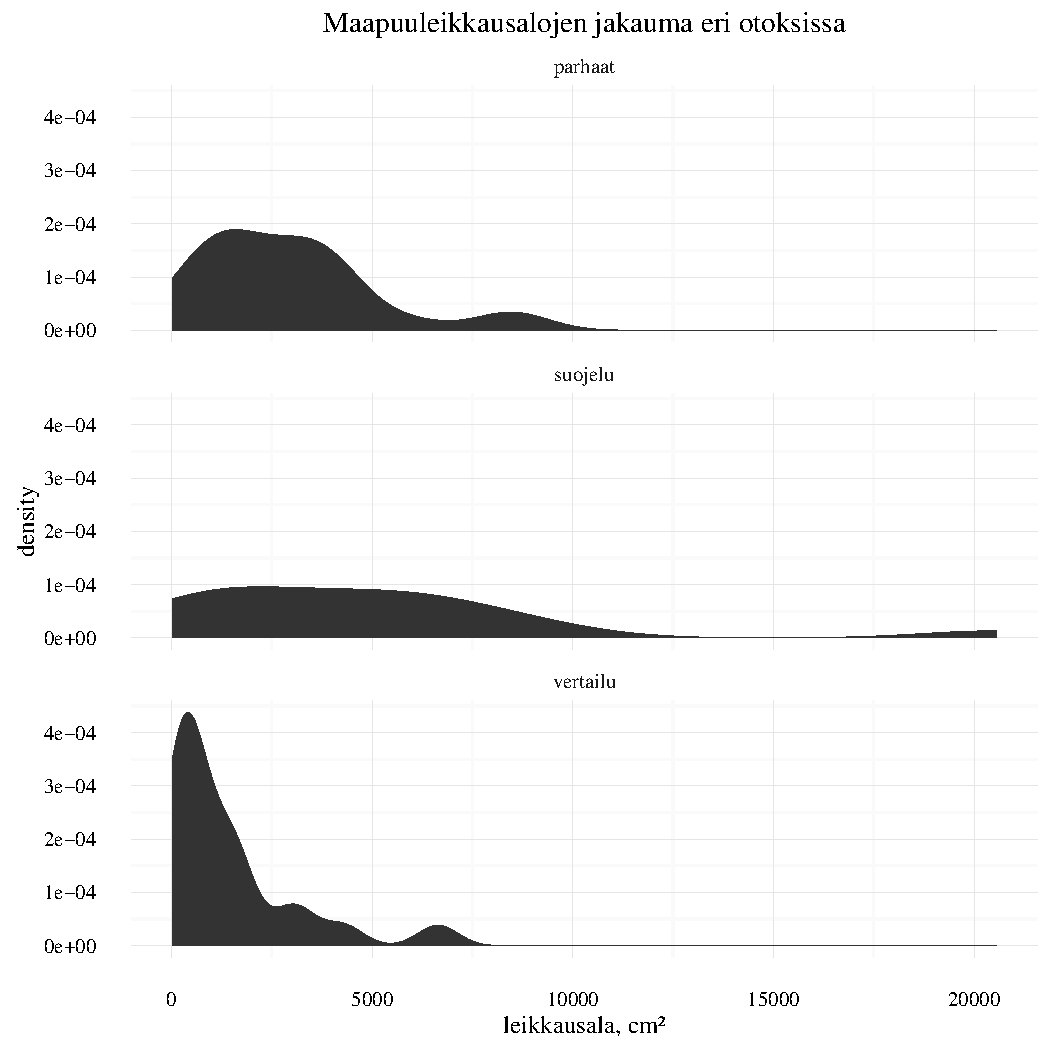
\includegraphics[height = 0.9\textheight]{maapuiden_leikkasalat.pdf}
  \end{center}
\end{frame}

\begin{frame}{Tulokset}
  \begin{center}
    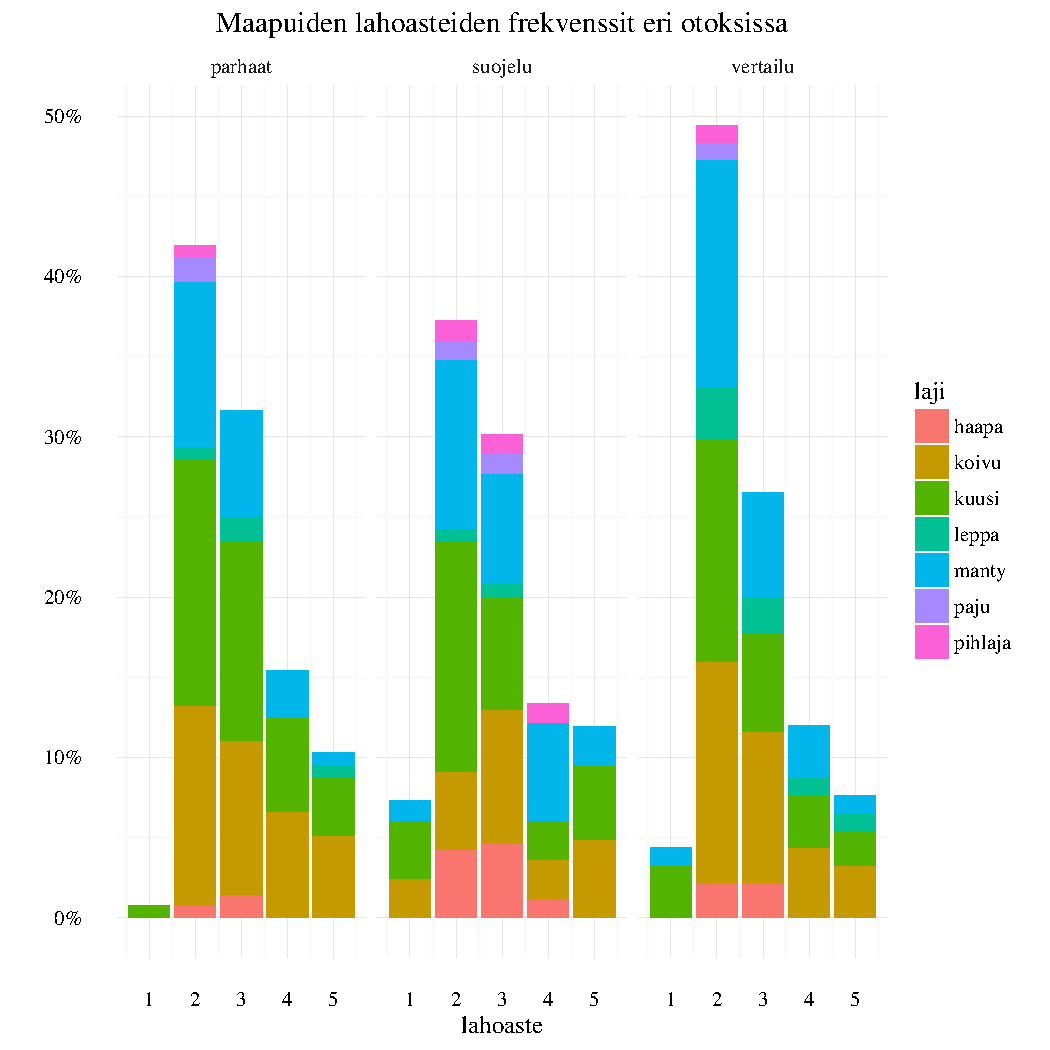
\includegraphics[height = 0.9\textheight]{lahoastefrekvenssit.pdf}
  \end{center}
\end{frame}

\begin{frame}{Tulokset}
  \begin{center}
    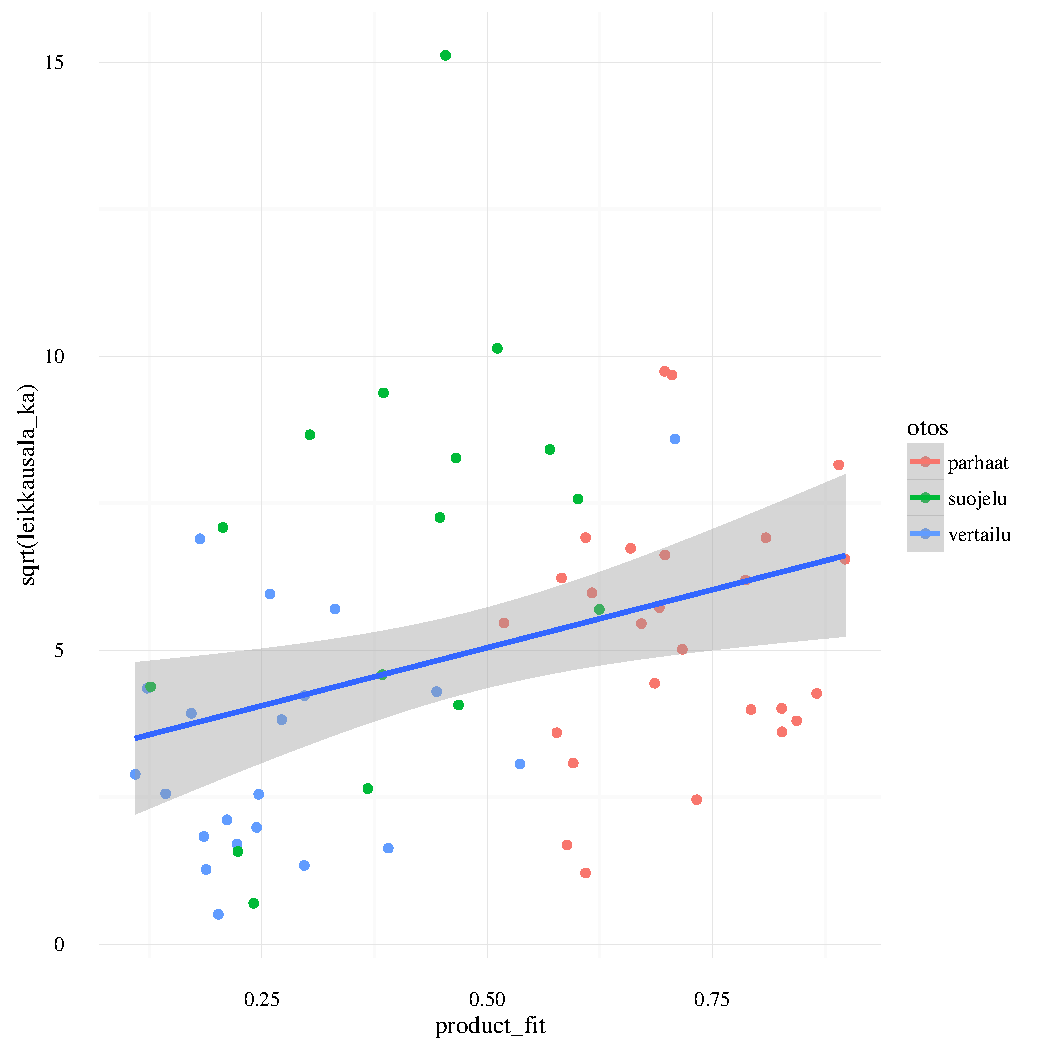
\includegraphics[height = 0.9\textheight]{vastaavus.pdf}
  \end{center}
\end{frame}

\begin{frame}{Tulokset}
Yksittäinen karttapiste ei ennusta lahopuurunsaita metsiä kovin hyvin.

Tilanne kuitenkin muuttuu, kun etsitään kartalta laajoja yhtenäisiä alueita, joille malli antaa korkeita arvoja.Tällöin mallin ennustemetsät ovat selvästi lähempänä suojelualueita lahopuusisällöltään kuin vertailumetsät.

Suojelualueilla on kuitenkin enemmän, pidemmälle lahonnutta ja lajikoostumukseltaan monipuolisempaa lahopuuta.

Validoinnissa ei kuitenkaan etsitty parhaita metsiä, vaan vain otos parhaista.
\end{frame}

\begin{frame}{Julkaisu}
  Projektin tuotokset kaikkien vapaasti käytettävissä
  
  \url{http://fi.okfn.org/projects/biodiversity-map/}

  \url{https://zenodo.org/record/163765}
\end{frame}

\end{document}
